\documentclass[11pt, oneside]{article}   	% use "amsart" instead of "article" for AMSLaTeX format
\usepackage{geometry}                		% See geometry.pdf to learn the layout options. There are lots.
\geometry{letterpaper}                   		% ... or a4paper or a5paper or ... 
%\geometry{landscape}                		% Activate for for rotated page geometry
%\usepackage[parfill]{parskip}    		% Activate to begin paragraphs with an empty line rather than an indent
\usepackage{graphicx}				% Use pdf, png, jpg, or eps� with pdflatex; use eps in DVI mode
								% TeX will automatically convert eps --> pdf in pdflatex		
\usepackage{amssymb}

\title{Watchboy State of Health}
\author{T. Shokair}
%\date{}							% Activate to display a given date or no date

\begin{document}
\maketitle
%\section{}
%\subsection{}
The document shows the detector rates given the various applied cuts.  The total livetime of the data is shown in Figure \ref{fig:LT}.
\begin{figure}[htbp] %  figure placement: here, top, bottom, or page
   \centering
   \includegraphics[scale=.75]{/Users/tshokair/Desktop/Work/watchboy/stateOfHealth/liveTime.pdf} 
   \caption{Individual and Integrated Livetimes as a function of month}
   \label{fig:LT}
\end{figure}

\section{Method}
Rates are determined based on a charge balance cut as defined by Nathaniel in the analysis template. This version is somewhat simplified, in that I not specifically calculating the charge balance for a specific events but am simply counting the number of contributing channels. \\

The data are grouped into time periods of a single month, and at the start of each month the code reads in the charge to single photoelectron conversion factors. Additionally, at the start of each month, pedestals in each channel are checked for an appropriate fit. If the fit is off, then those specific channels are removed from the analysis. \\

The code then loops over every event in a run to count 7 quantities: 1) the total number of event 2) the total number of target events where 2 or more channels contribute ($>$1PMT target) 3) the total number of target events where 3 or more channels contribute ($>$2 PMT target) 4)  the total number of veto events where 1 or more channels contribute ($>$1PMT veto) 5) the total number of veto events where 2 or more channels contribute ($>$2PMT target) 6) the total number of events where EITHER 2 or more target channels contribute OR 2 or more veto channels contribute ($>$1 PMT Either) 7)the total number of events where BOTH 2 or more target channels contribute AND 2 or more veto channels contribute ($>$1 PMT Both) . Rates are then calculated by dividing the total number of event given a specific cut by the total run time. \\

Additionally quantities tracking individual channels over time are calculated and used to check runs with anomalous rates. 
\section{The Plots}
Below are the plots of event rates as a function of time, with one plot for each calendar month of data.
\begin{figure}[htbp] %  figure placement: here, top, bottom, or page
   \centering
   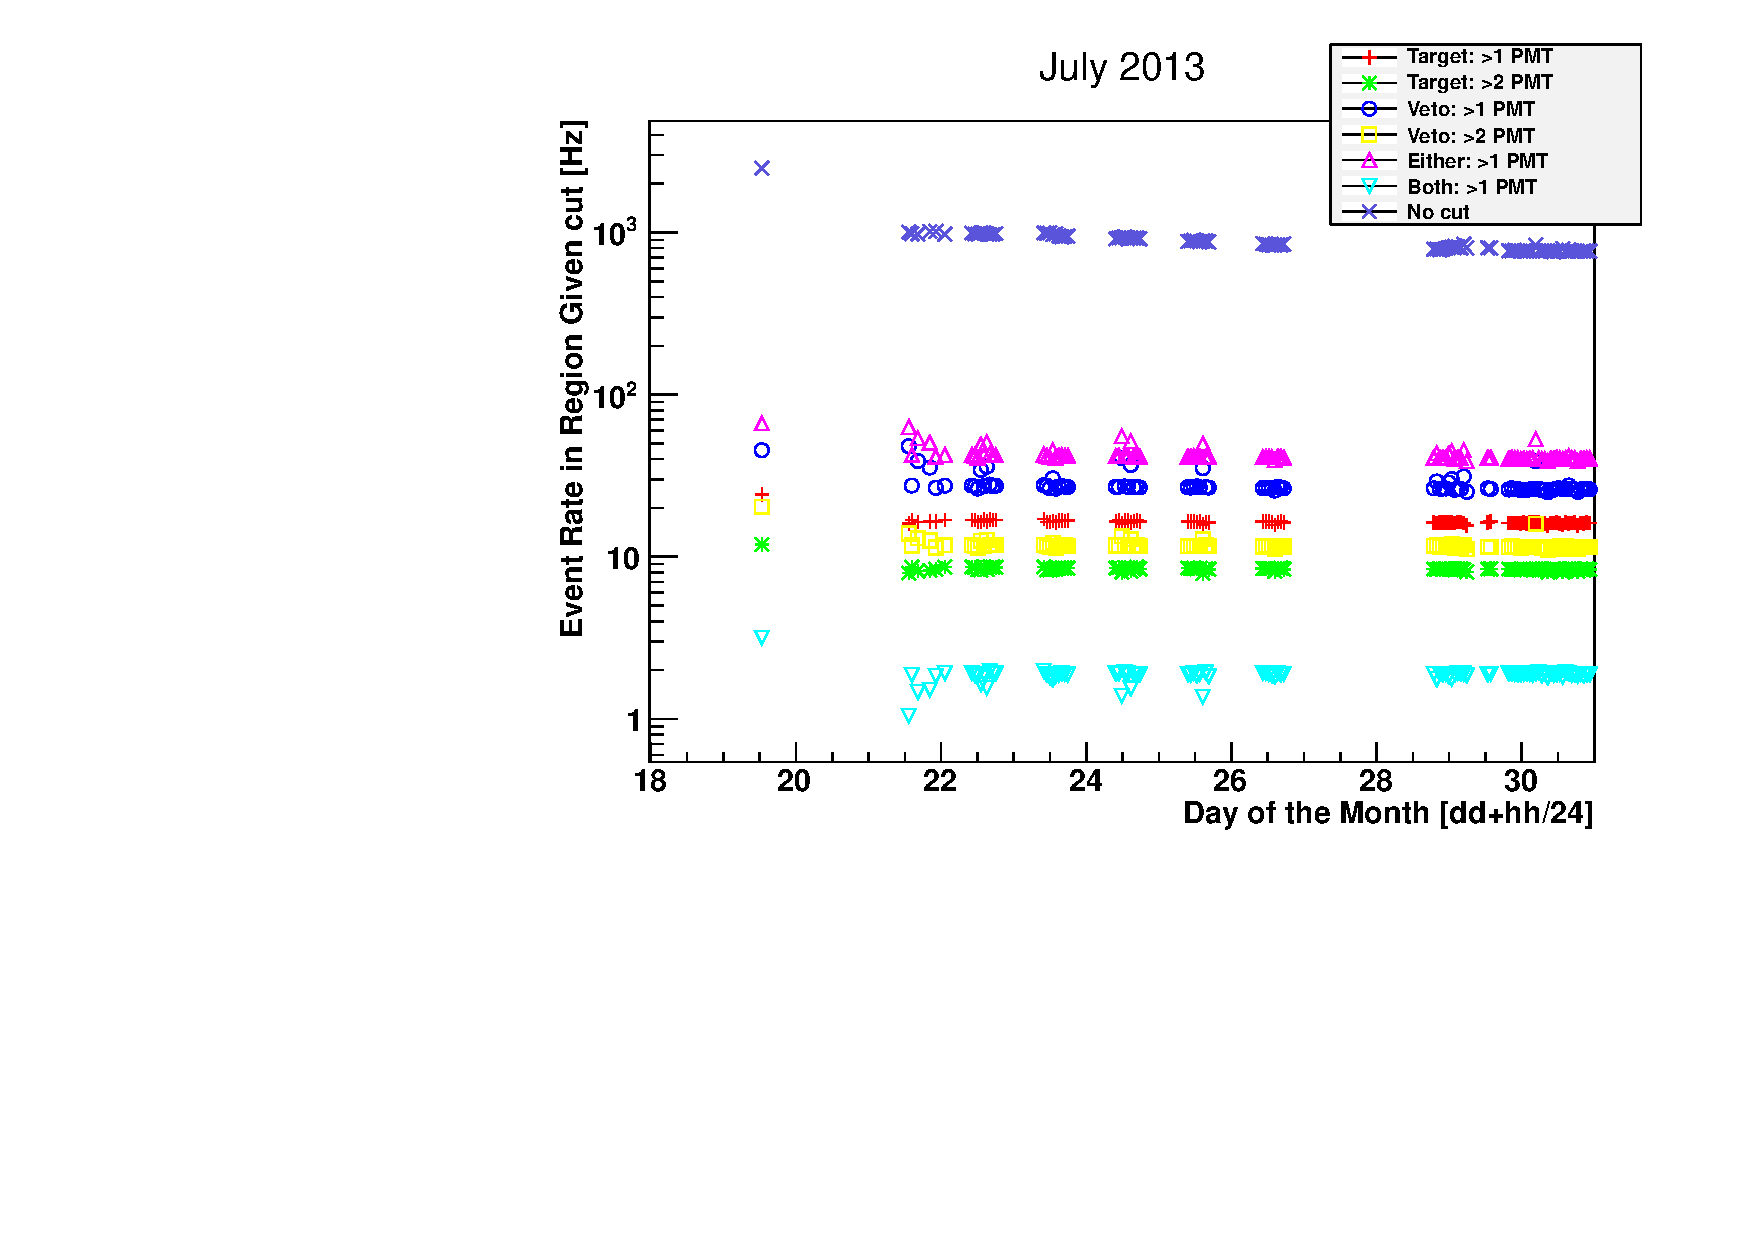
\includegraphics[scale=.75]{/Users/tshokair/Desktop/Work/watchboy/SOH/plotsPDF/y13m07EventRates_Scatter.pdf} 
   \caption{Events Rates in July}
   \label{fig:july13}
\end{figure}

\begin{figure}[htbp] %  figure placement: here, top, bottom, or page
   \centering
   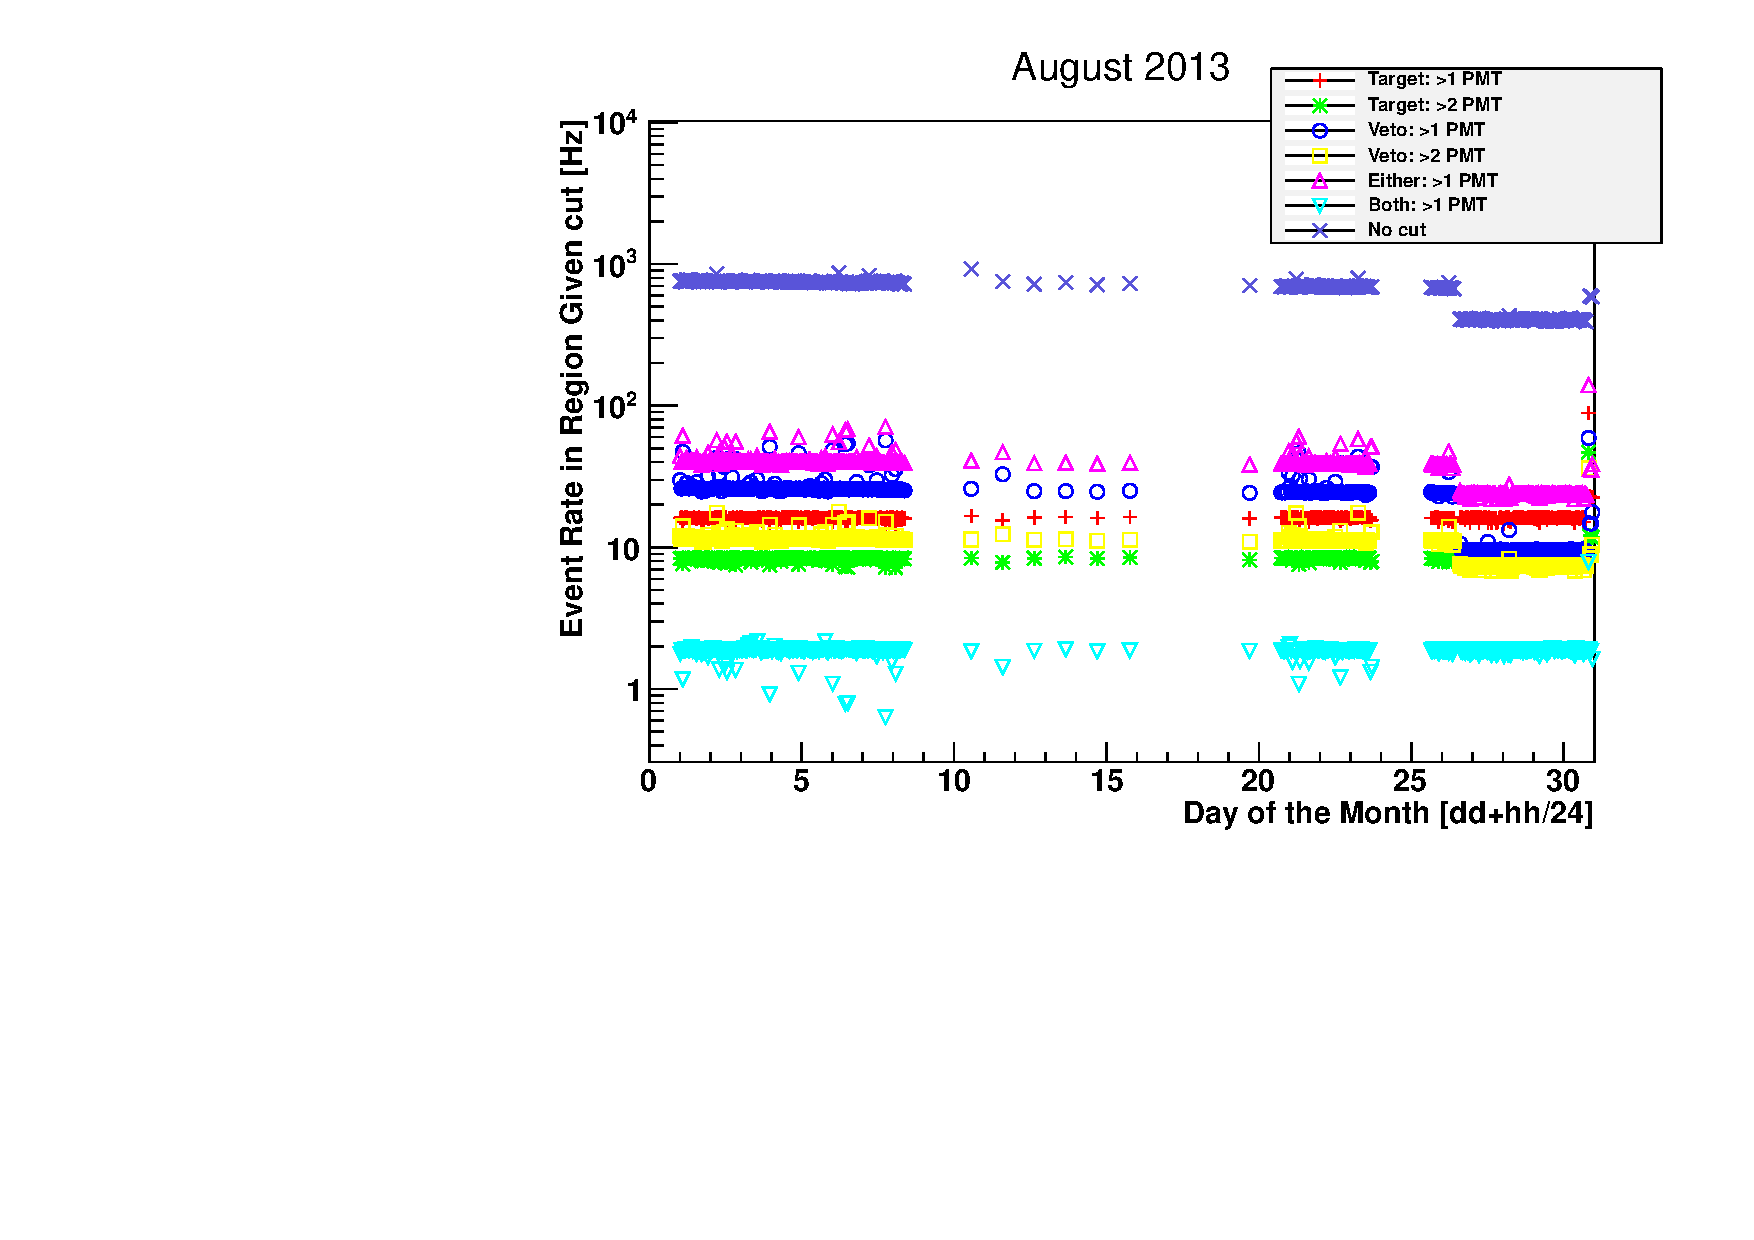
\includegraphics[scale=.75]{/Users/tshokair/Desktop/Work/watchboy/SOH/plotsPDF/y13m08EventRates_Scatter.pdf} 
   \caption{Events Rates in August}
   \label{fig:aug13}
\end{figure}

\begin{figure}[htbp] %  figure placement: here, top, bottom, or page
   \centering
   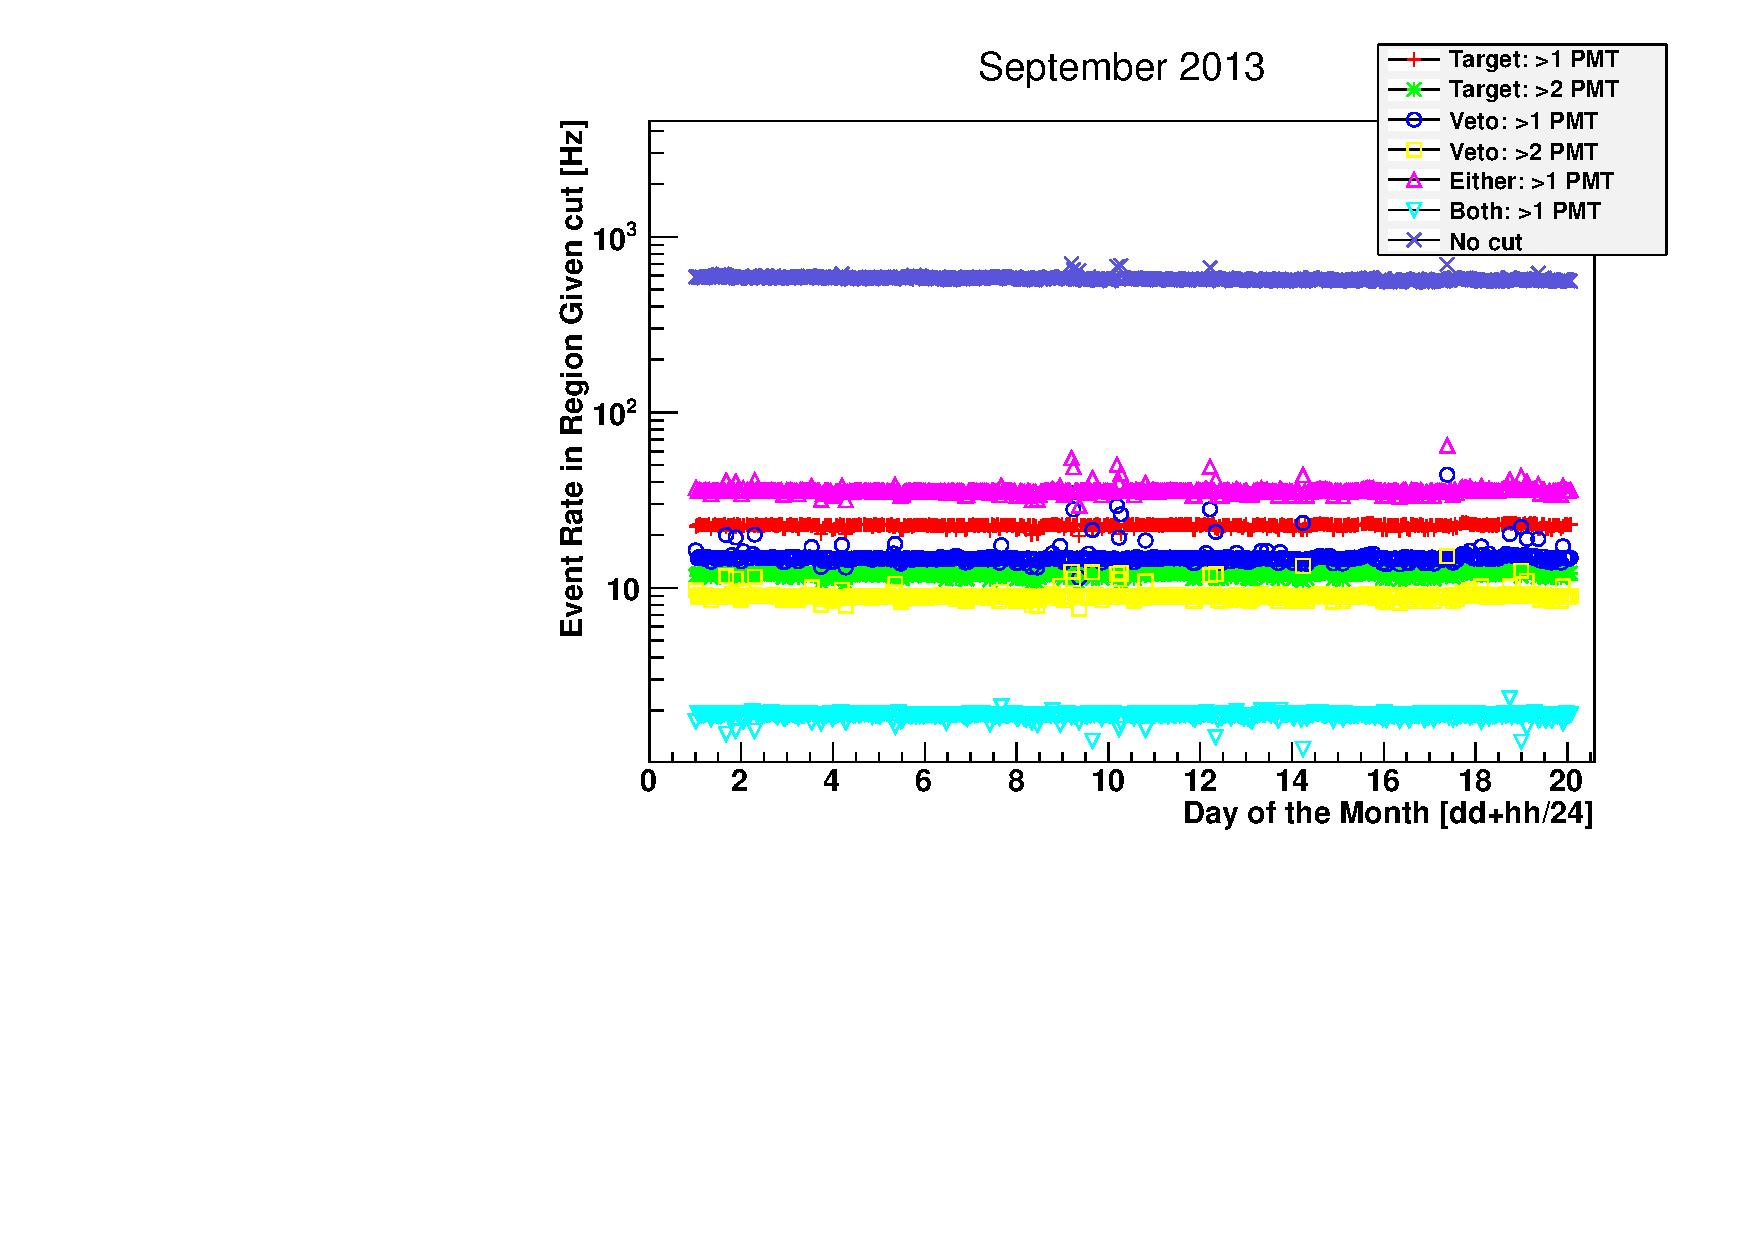
\includegraphics[scale=.75]{/Users/tshokair/Desktop/Work/watchboy/SOH/plotsPDF/y13m09EventRates_Scatter.pdf} 
   \caption{Events Rates in September}
   \label{fig:sep13}
\end{figure}
\begin{figure}[htbp] %  figure placement: here, top, bottom, or page
   \centering
   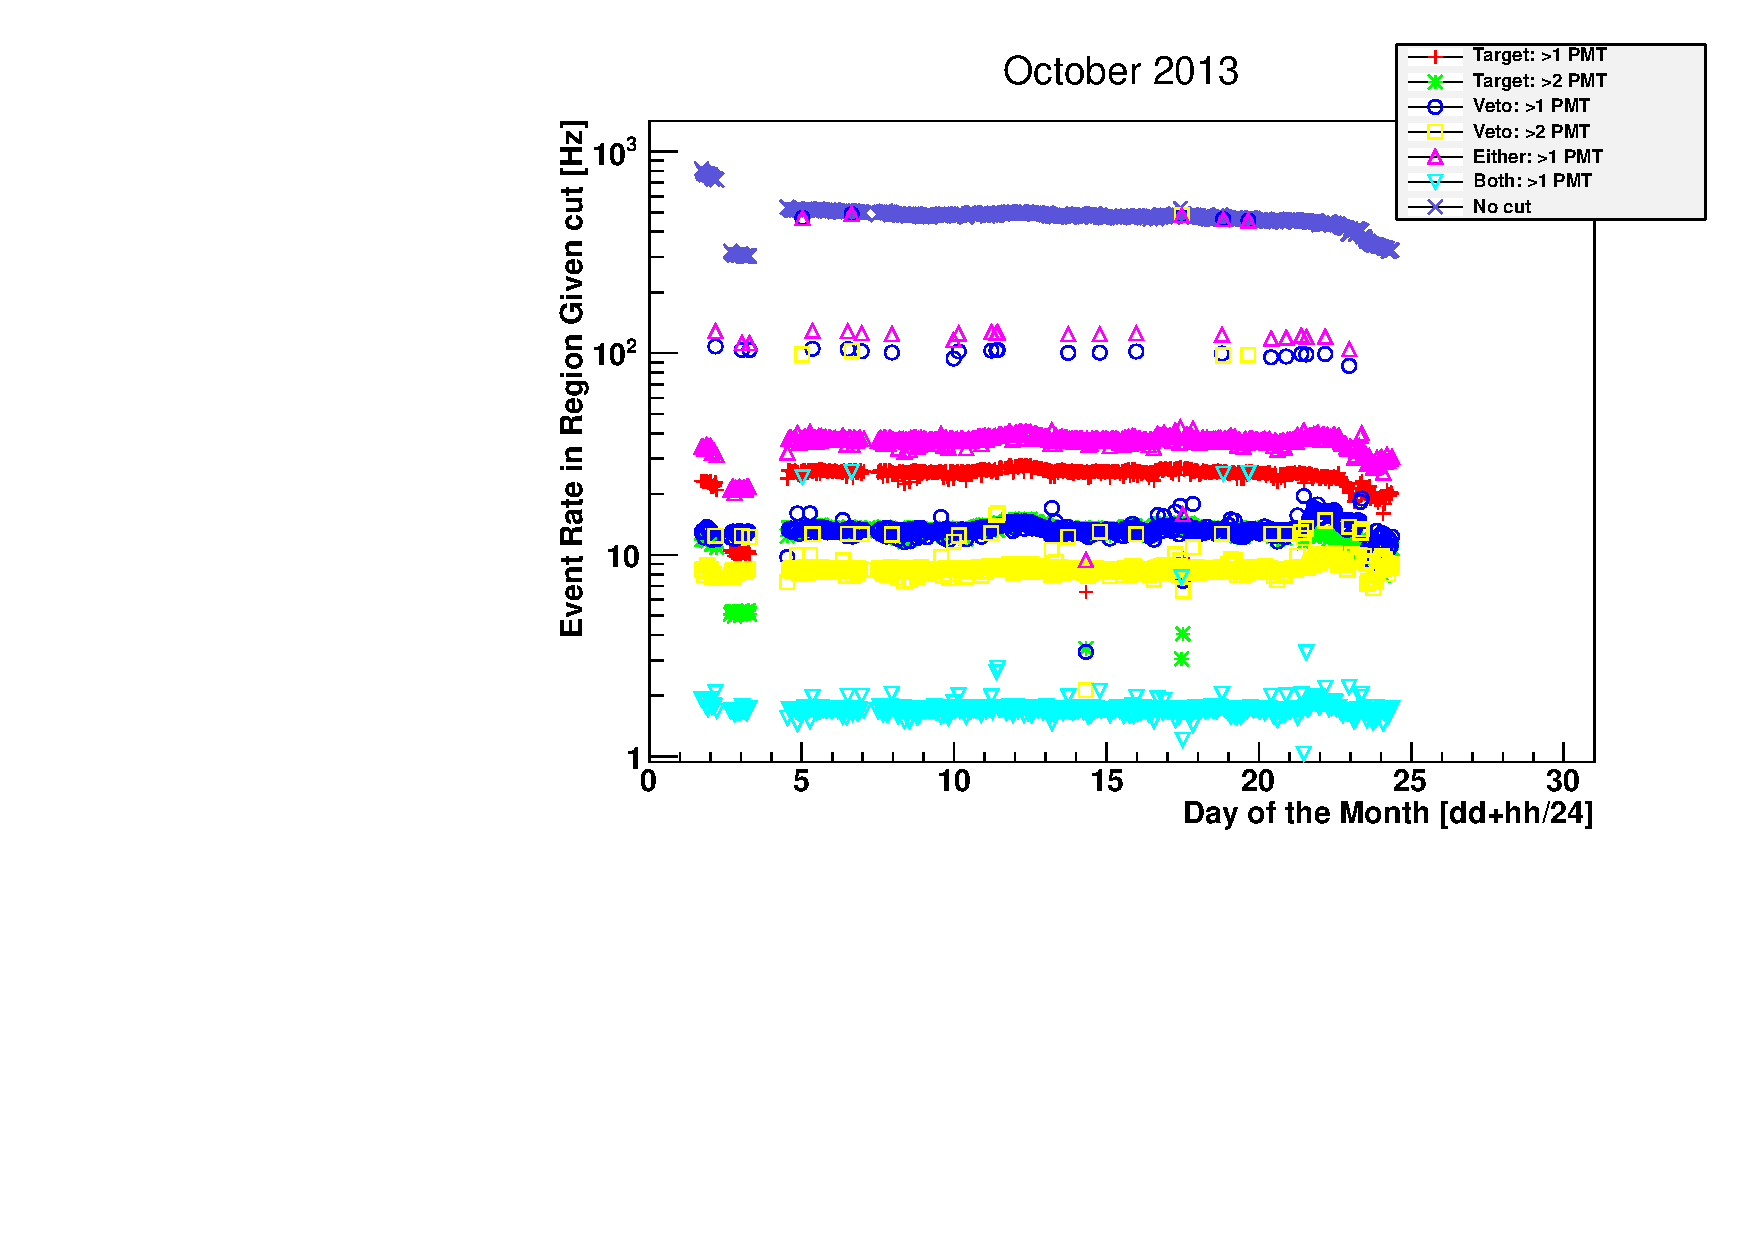
\includegraphics[scale=.75]{/Users/tshokair/Desktop/Work/watchboy/SOH/plotsPDF/y13m10EventRates_Scatter.pdf} 
   \caption{Events Rates in October}
   \label{fig:oct13}
\end{figure}

\begin{figure}[htbp] %  figure placement: here, top, bottom, or page
   \centering
   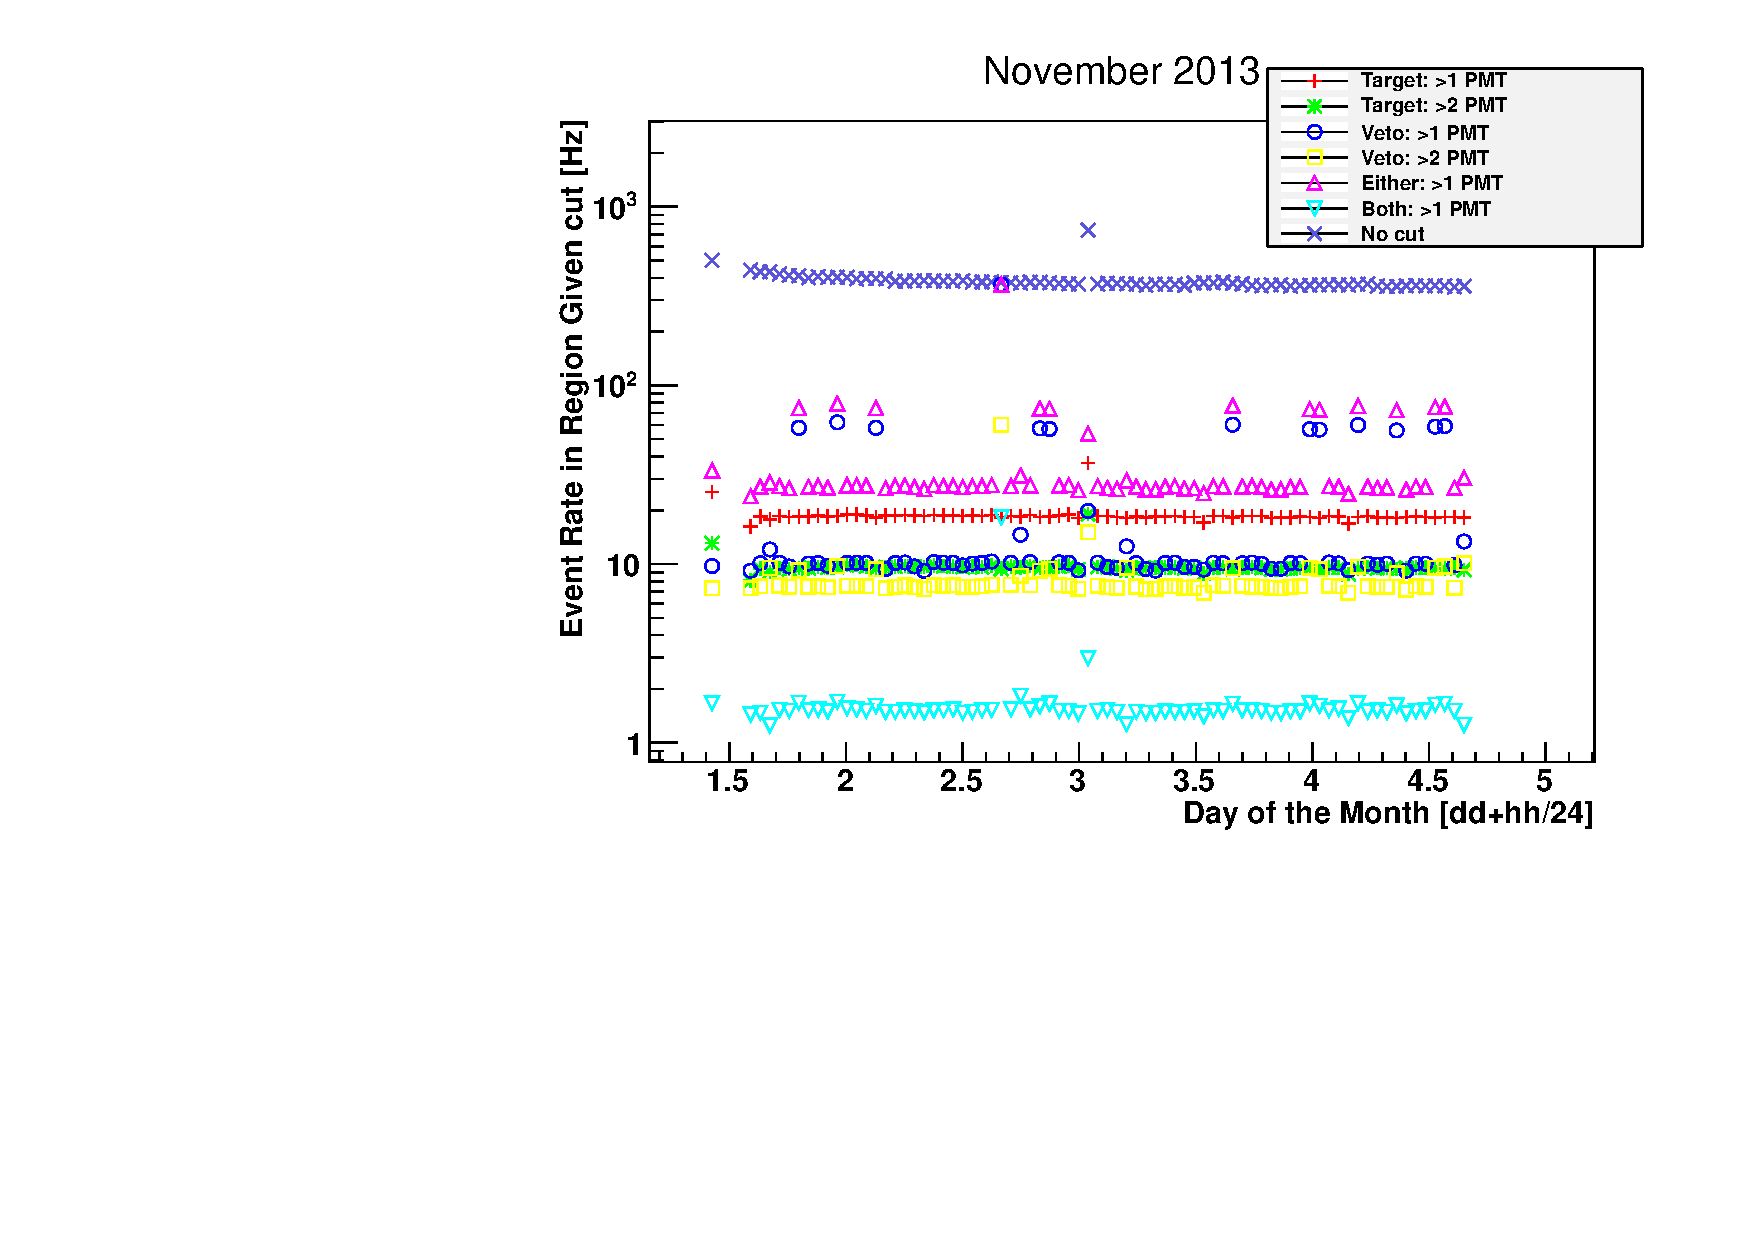
\includegraphics[scale=.75]{/Users/tshokair/Desktop/Work/watchboy/SOH/plotsPDF/y13m11EventRates_Scatter.pdf} 
   \caption{Events Rates in November}
   \label{fig:nov13}
\end{figure}

\begin{figure}[htbp] %  figure placement: here, top, bottom, or page
   \centering
   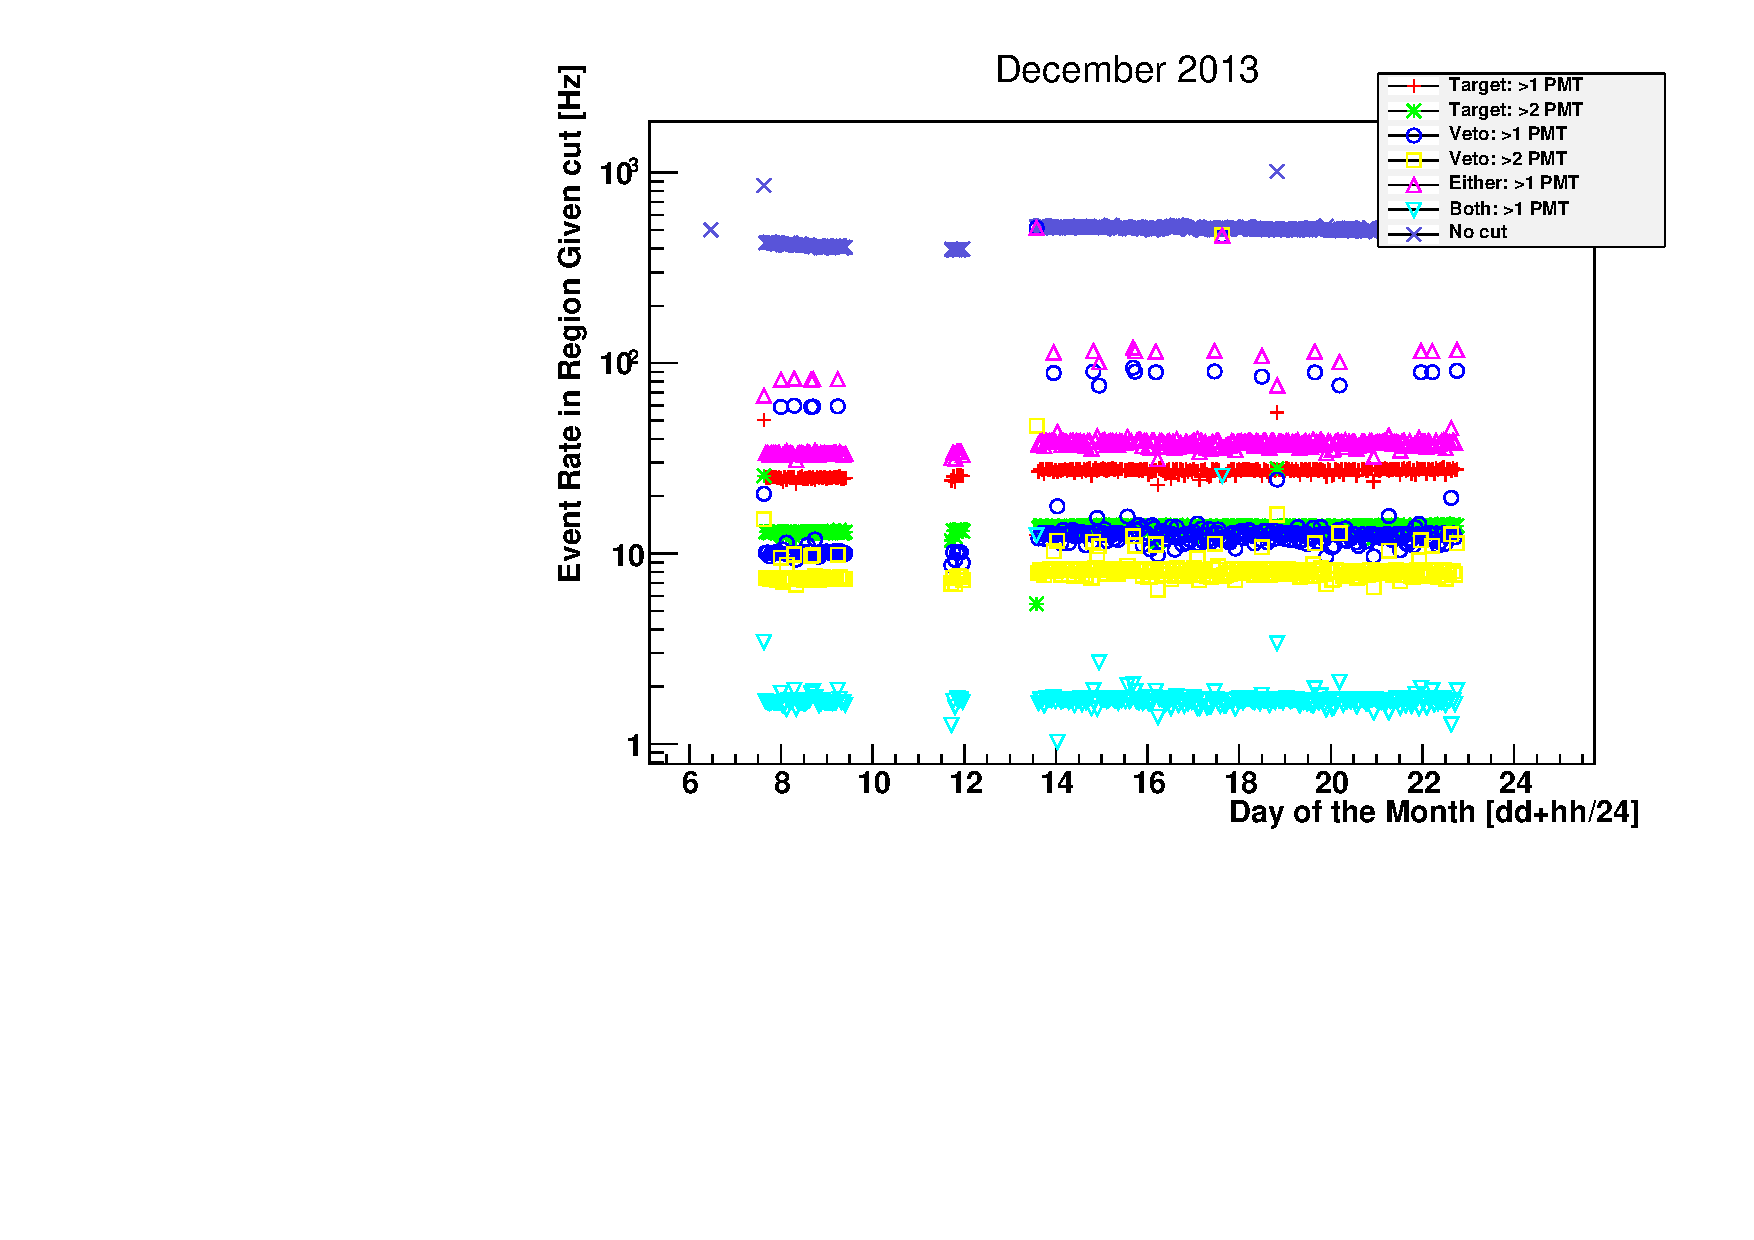
\includegraphics[scale=.75]{/Users/tshokair/Desktop/Work/watchboy/SOH/plotsPDF/y13m12EventRates_Scatter.pdf} 
   \caption{Events Rates in December}
   \label{fig:dec13}
\end{figure}
\begin{figure}[htbp] %  figure placement: here, top, bottom, or page
   \centering
   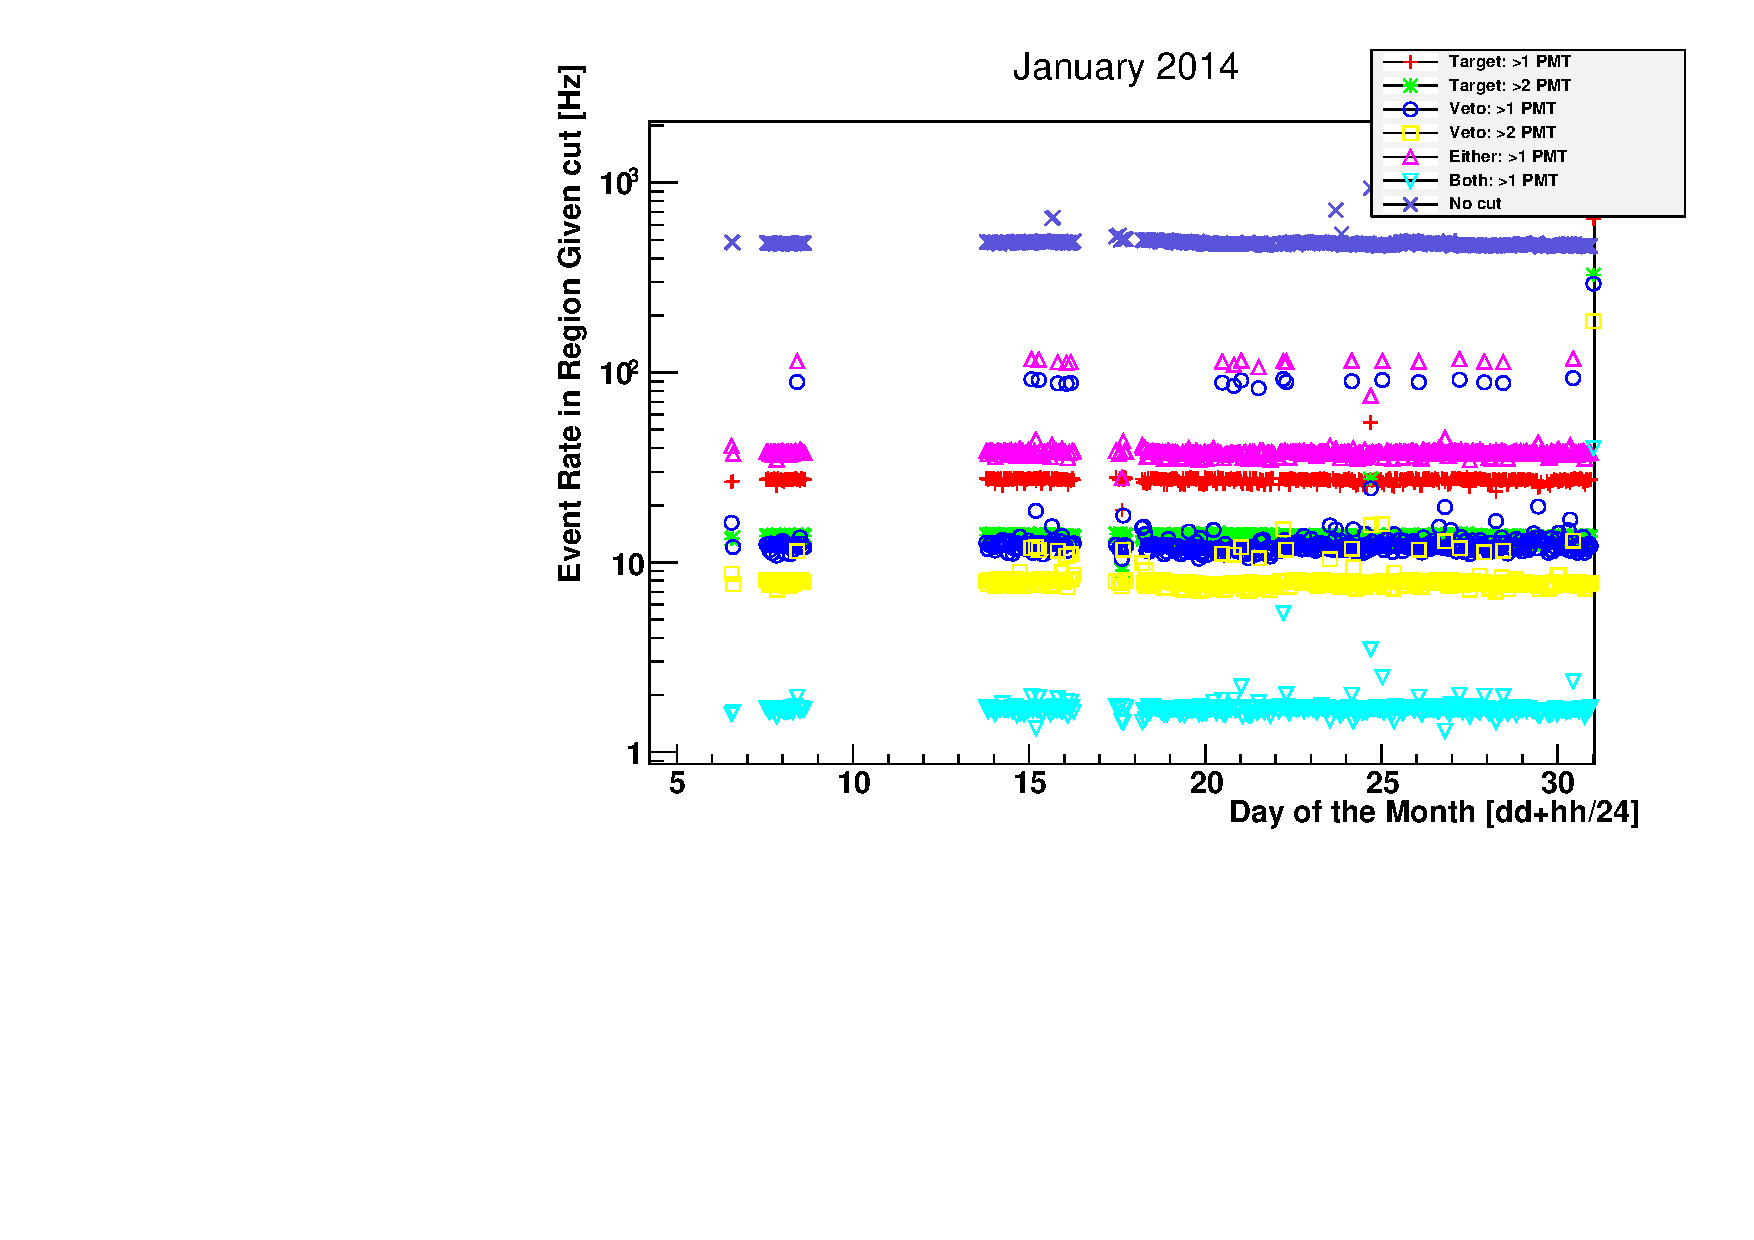
\includegraphics[scale=.75]{/Users/tshokair/Desktop/Work/watchboy/SOH/plotsPDF/y14m01EventRates_Scatter.pdf} 
   \caption{Events Rates in January 14}
   \label{fig:jan14}
\end{figure}
\begin{figure}[htbp] %  figure placement: here, top, bottom, or page
   \centering
   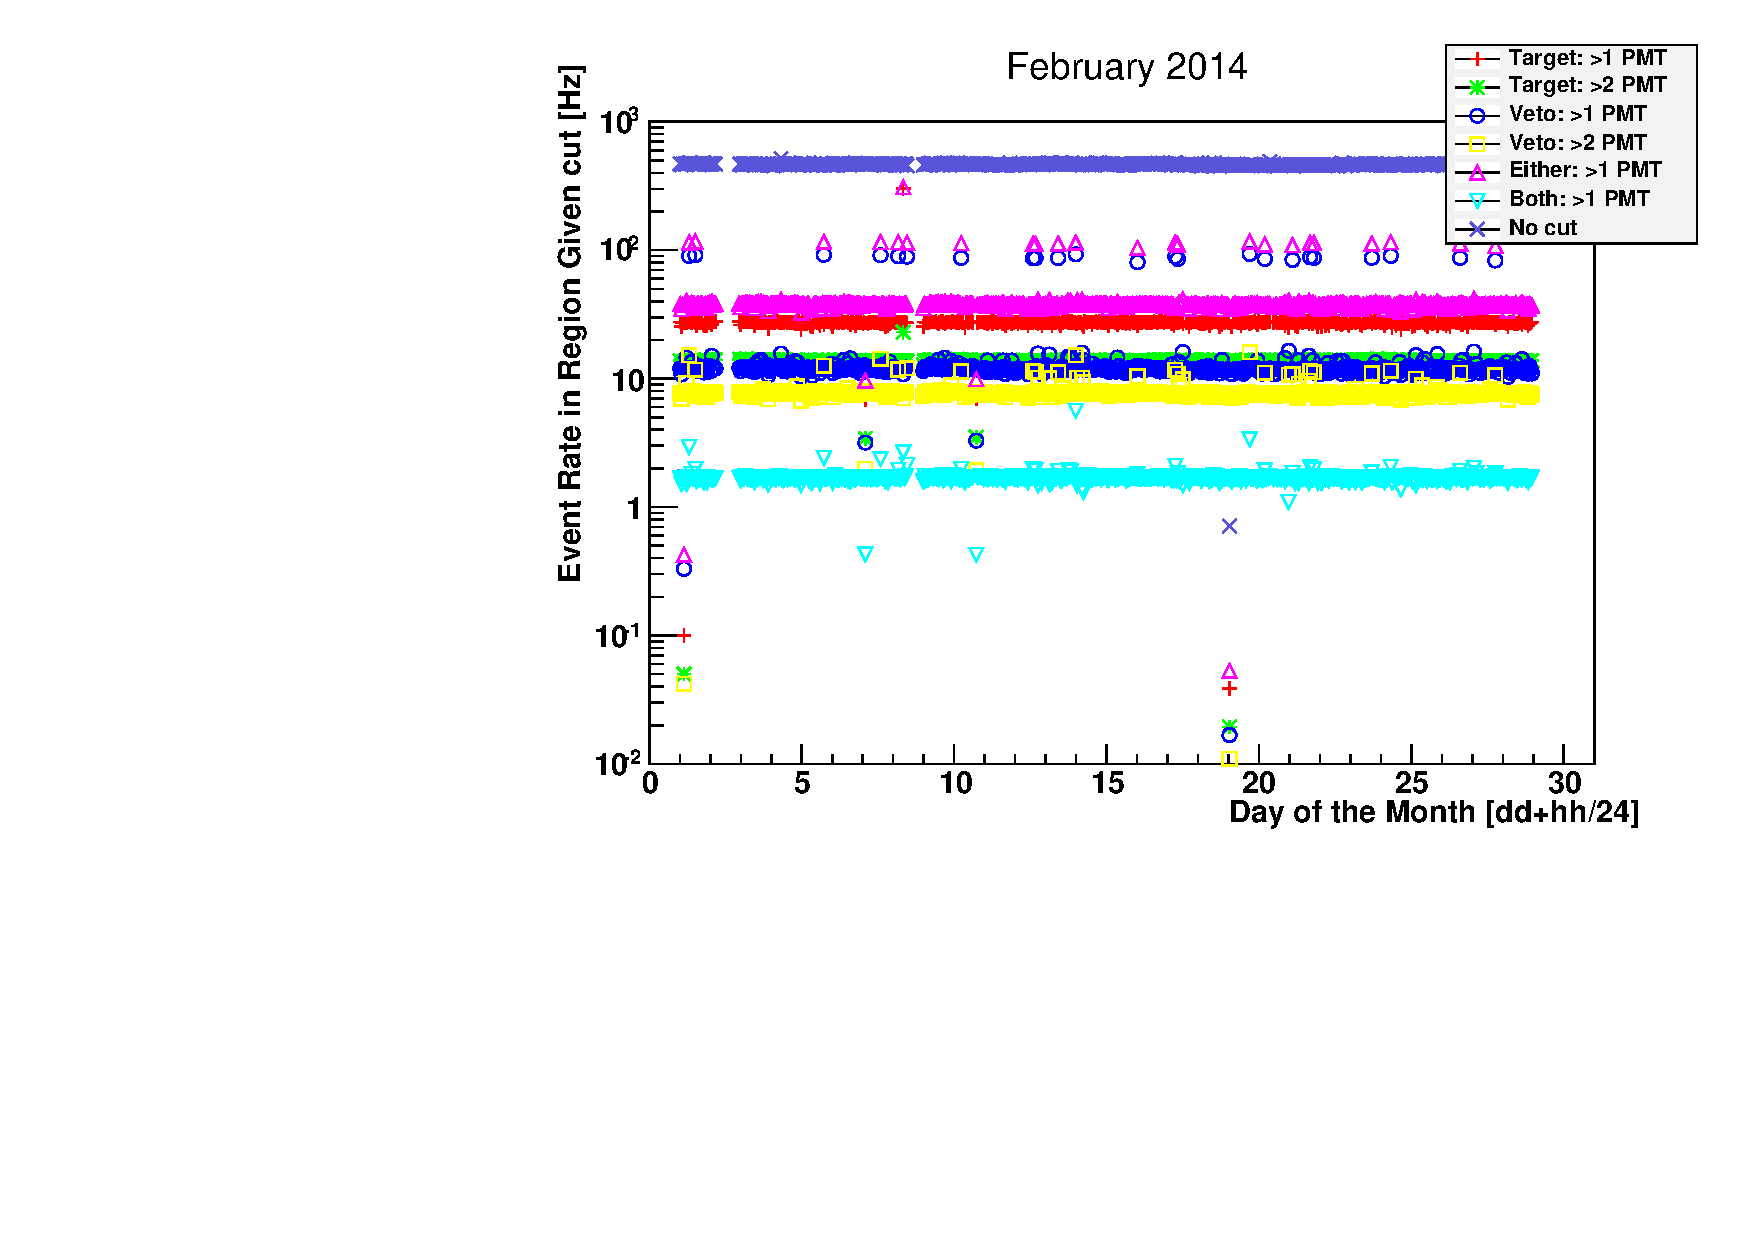
\includegraphics[scale=.75]{/Users/tshokair/Desktop/Work/watchboy/SOH/plotsPDF/y14m02EventRates_Scatter.pdf} 
   \caption{Events Rates in February 14}
   \label{fig:feb14}
\end{figure}
\begin{figure}[htbp] %  figure placement: here, top, bottom, or page
   \centering
   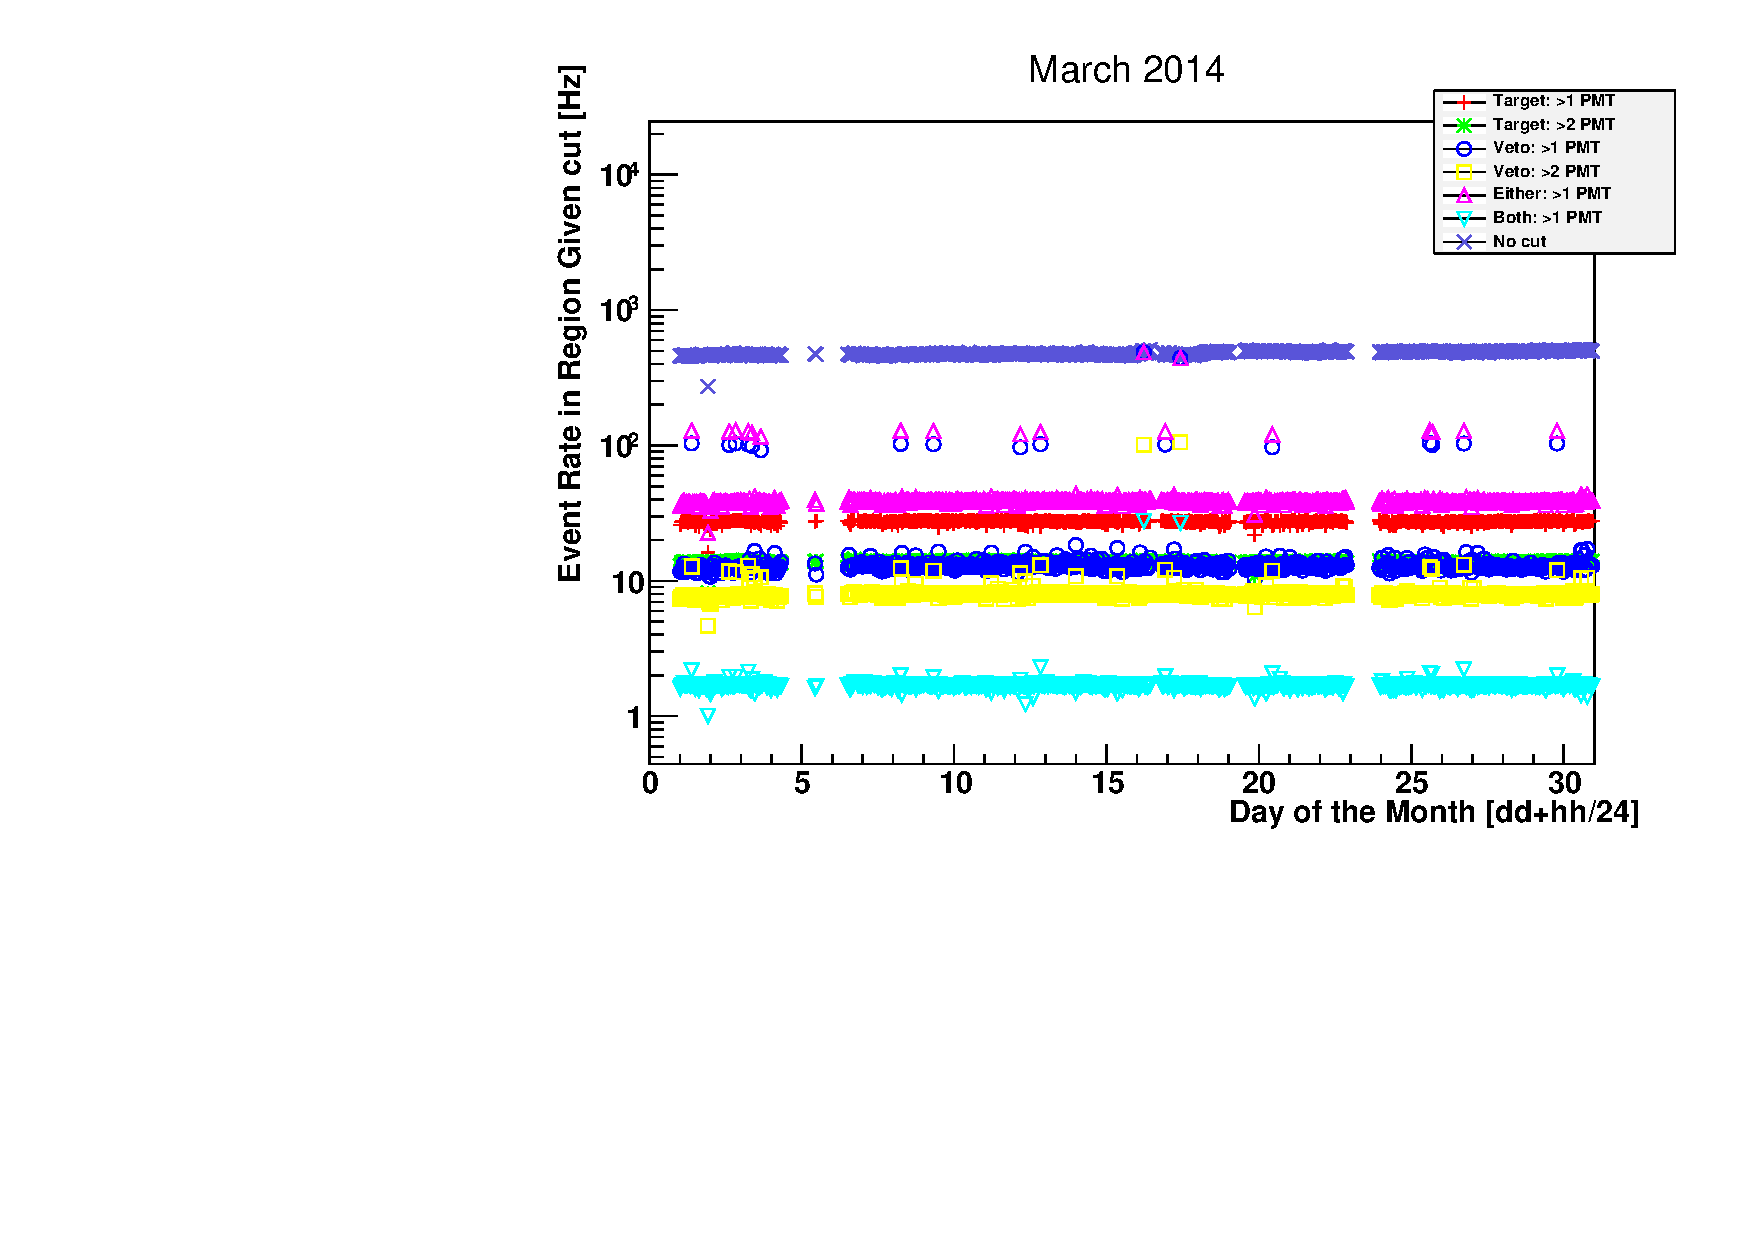
\includegraphics[scale=.75]{/Users/tshokair/Desktop/Work/watchboy/SOH/plotsPDF/y14m03EventRates_Scatter.pdf} 
   \caption{Events Rates in March 14}
   \label{fig:mar14}
\end{figure}

\begin{figure}[htbp] %  figure placement: here, top, bottom, or page
   \centering
   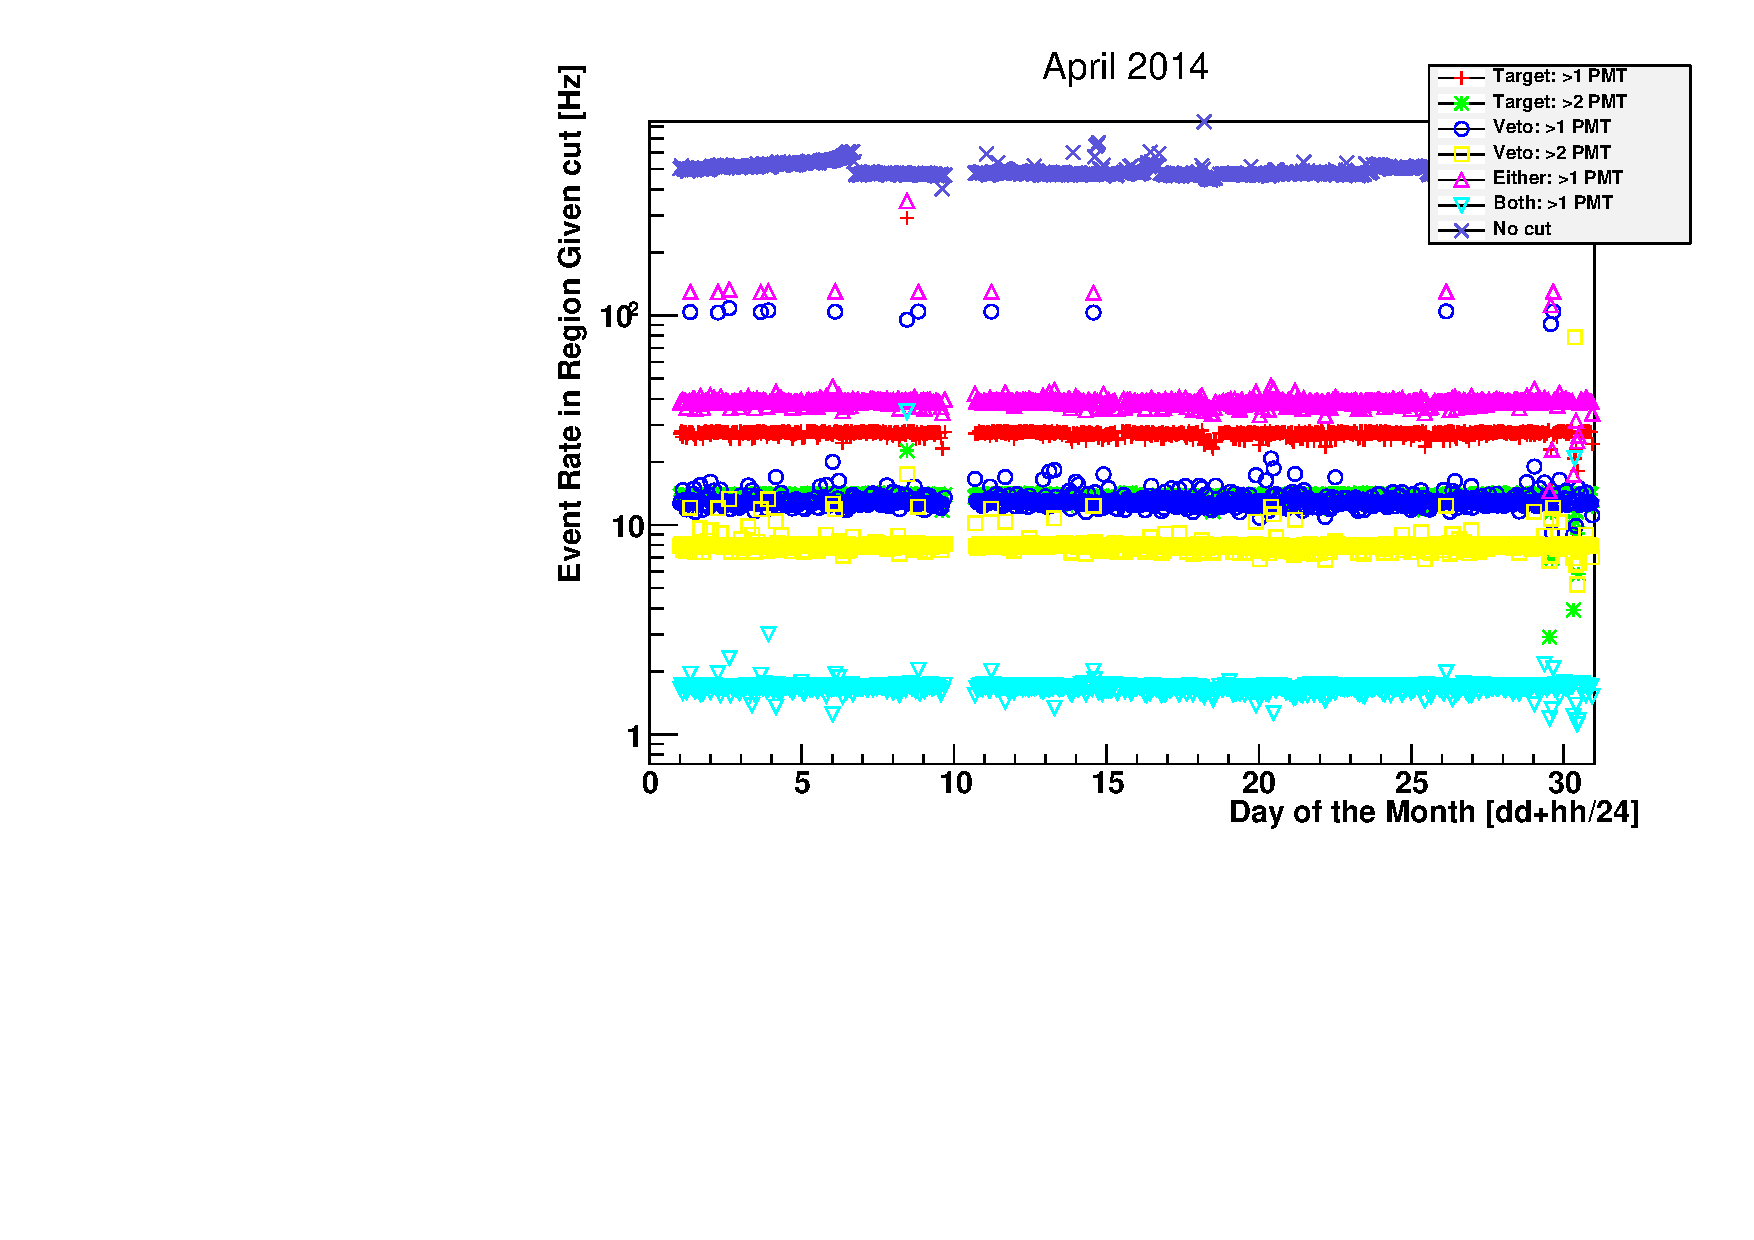
\includegraphics[scale=.75]{/Users/tshokair/Desktop/Work/watchboy/SOH/plotsPDF/y14m04EventRates_Scatter.pdf} 
   \caption{Events Rates in April 14}
   \label{fig:apl14}
\end{figure}

\begin{figure}[htbp] %  figure placement: here, top, bottom, or page
   \centering
   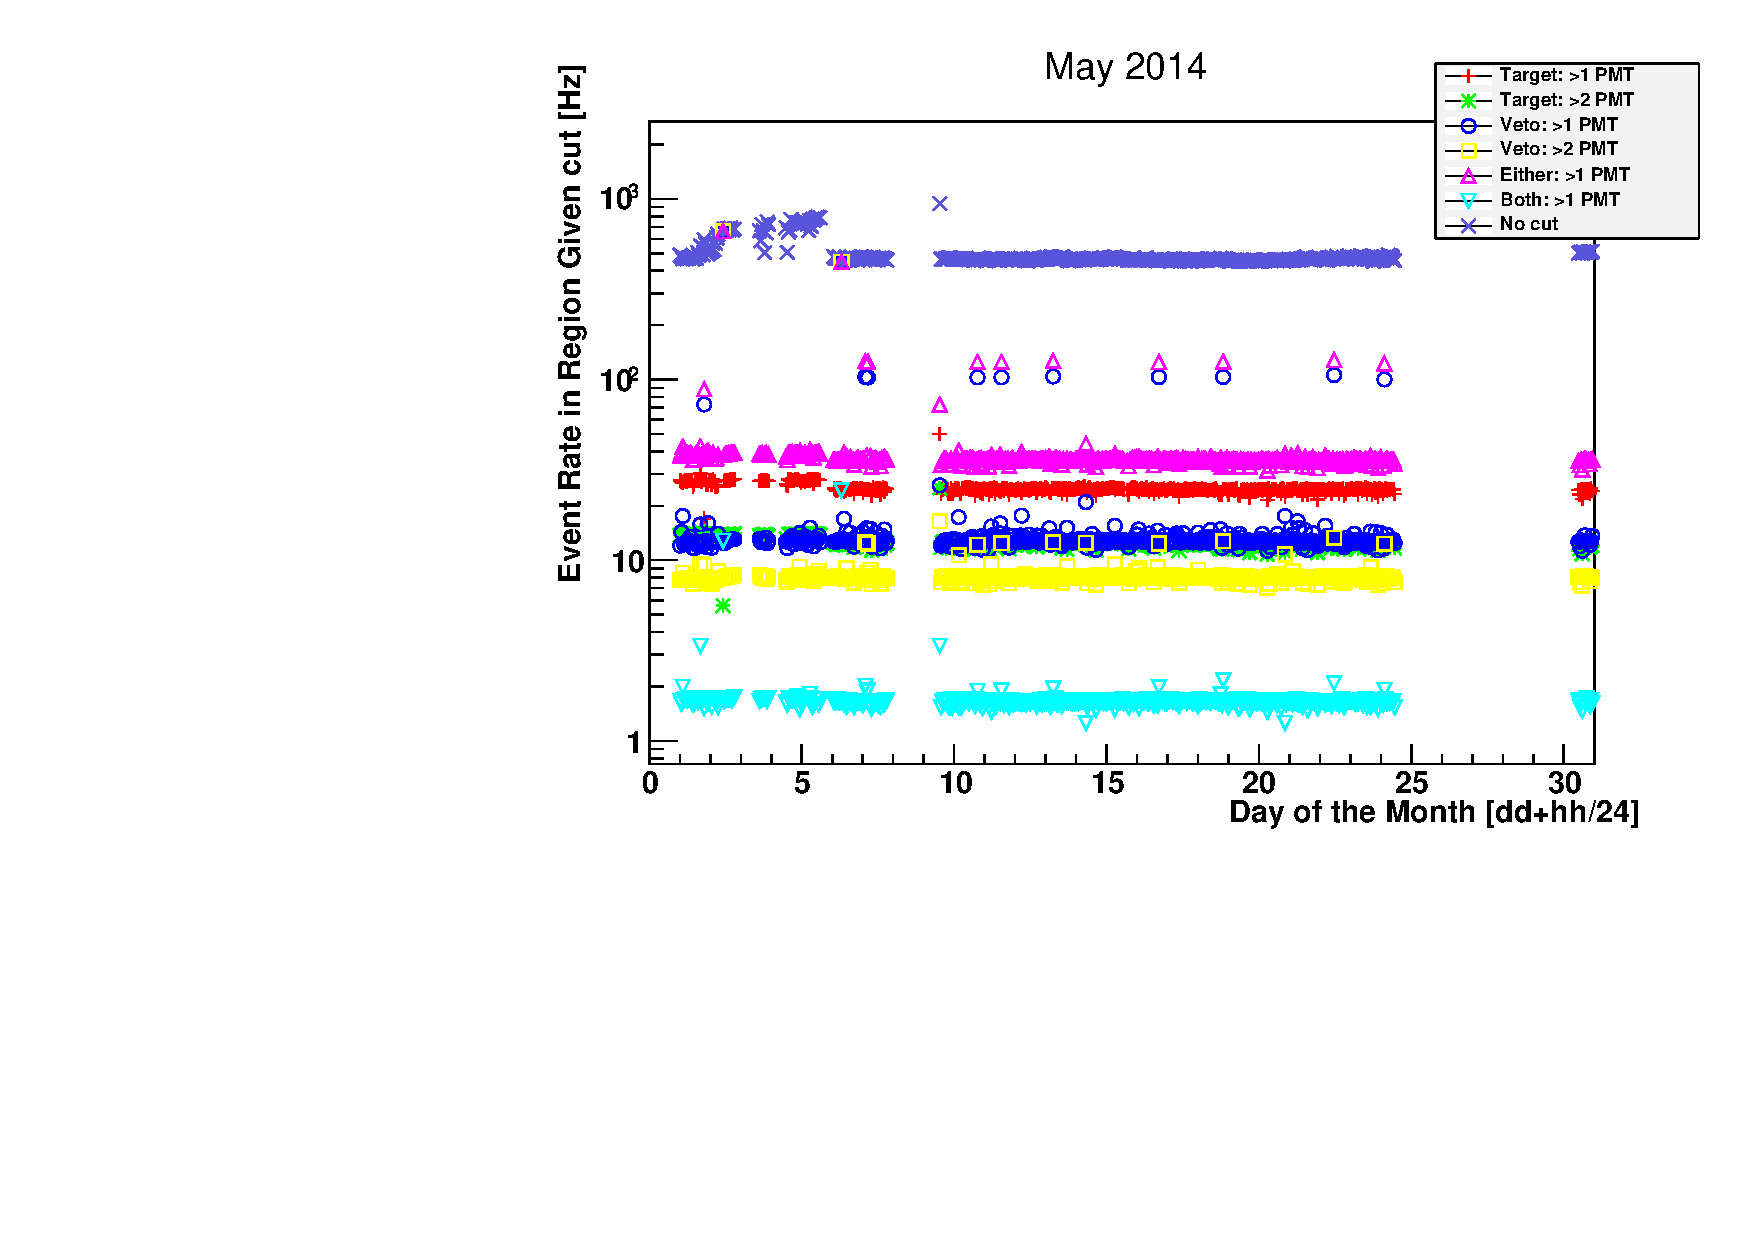
\includegraphics[scale=.75]{/Users/tshokair/Desktop/Work/watchboy/SOH/plotsPDF/y14m05EventRates_Scatter.pdf} 
   \caption{Events Rates in May 14}
   \label{fig:may14}
\end{figure}

\begin{figure}[htbp] %  figure placement: here, top, bottom, or page
   \centering
   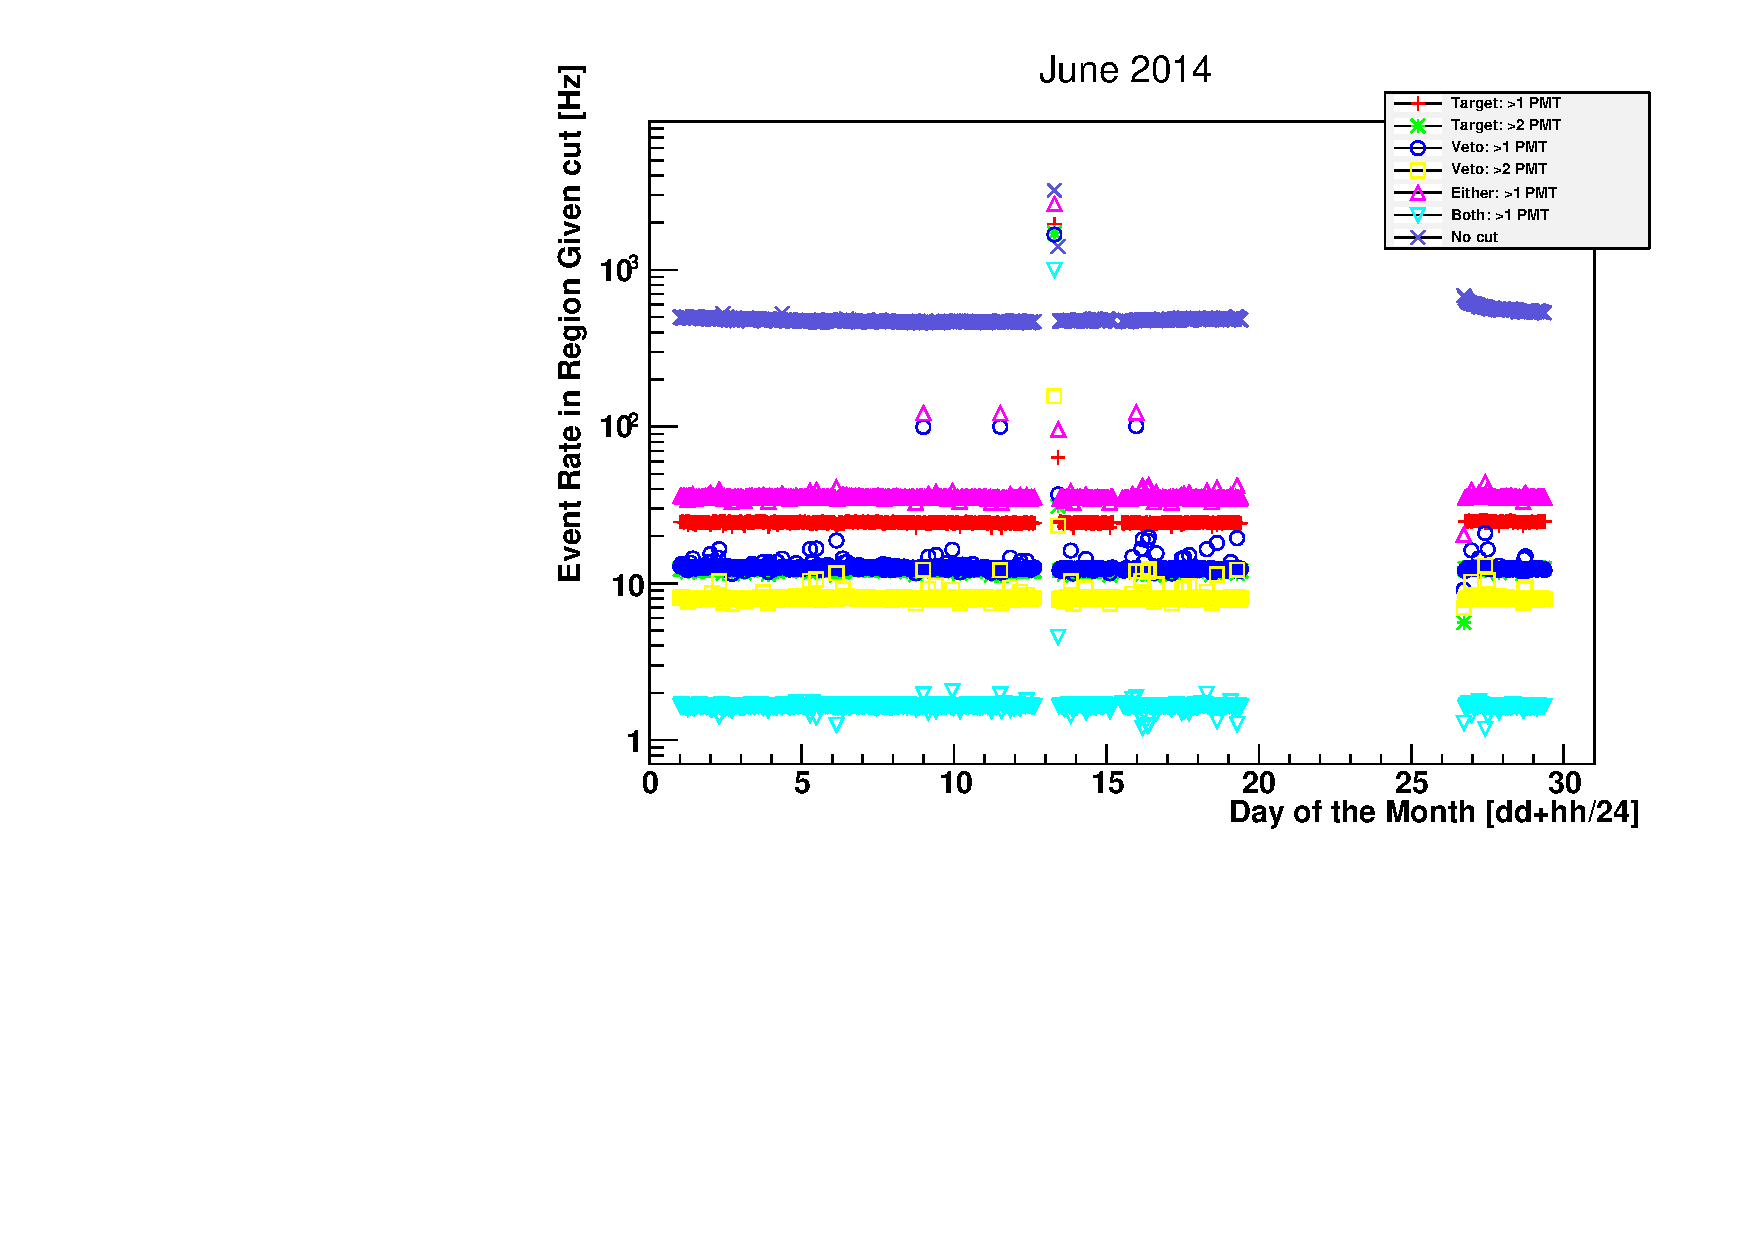
\includegraphics[scale=.75]{/Users/tshokair/Desktop/Work/watchboy/SOH/plotsPDF/y14m06EventRates_Scatter.pdf} 
   \caption{Events Rates in June14}
   \label{fig:jun14}
\end{figure}



\end{document}  
